\documentclass[a4paper,12pt]{article}

\usepackage{graphicx} % Required for inserting images
\usepackage{amsmath,amssymb,amsfonts}
\usepackage{subcaption}
% -----------------------
% Package Imports
% -----------------------

% Set page margins
\usepackage[a4paper, top=1in, bottom=0.8in, left=1.1in, right=0.8in]{geometry}

% Use Times New Roman font
\usepackage{times}
\usepackage{array}


% Add page numbering
\pagestyle{plain}
\usepackage{multirow}
% Enable graphics inclusion
\usepackage{graphicx}
\usepackage{float}
% Enable code listings
\usepackage{listings}
\usepackage{xcolor} % For customizing code colors

% Define MATLAB style for listings
\lstdefinestyle{vscode-light}{
	language=Matlab,
	basicstyle=\ttfamily\footnotesize,
	keywordstyle=\color{black},
	commentstyle=\color{gray},
	stringstyle=\color{red},
	numberstyle=\tiny\color{black},
	numbersep=5pt,
	frame=single,
	backgroundcolor=\color{white!10},
	breaklines=true,
	captionpos=b,
	tabsize=4,
	showstringspaces=false,
	numbers=left,  % Enable line numbering on the left
	stepnumber=1,  % Line numbers increment by 1
	numberfirstline=true, % Number the first line
}
\setlength{\parindent}{0pt}
\usepackage{titlesec} % To customize section font size
\titleformat{\section}
{\normalfont\fontsize{14}{16}\bfseries}{\thesection}{1em}{}

\titleformat{\subsection}
{\normalfont\fontsize{14}{16}\bfseries}{\thesubsection}{1em}{}


\begin{document}
	\section{Experiment No. 6}
	
	\section{Experiment Title }
	Observation \& Verification of Various Signals in Telecommunication Network.


	\section{Objectives}
	The objectives of this experiment are:
	\begin{itemize}
		\item To understand the working principle of a Telephone Set Trainer Module.
		\item To identify and examine dial tone, ring tone, busy tone, and speech signals.
		\item To analyze signal flow during call setup and termination using a designated IP address.
		\item To study the transmission and reception of audio signals through telephone lines.
		\item To verify and interpret various signals in a telephone network using LVTTS.
	\end{itemize}
	
	\section{Theory}
		This experiment focuses on understanding and verifying the various signals present in telecommunication networks, particularly in traditional telephone systems. The practical observations help demonstrate the fundamental principles of call setup, maintenance, and termination in Public Switched Telephone Networks (PSTN).
	
	Modern telephone sets use electronic circuits instead of large mechanical bells. The ringing sound is generated by a sound transducer driven by these circuits. When a call is initiated, an AC ringing voltage from the exchange is sent through a ring generator and activates the ringer circuit of the callee's telephone, causing it to ring until answered or canceled.
	
	\begin{figure}[H]
		\centering
	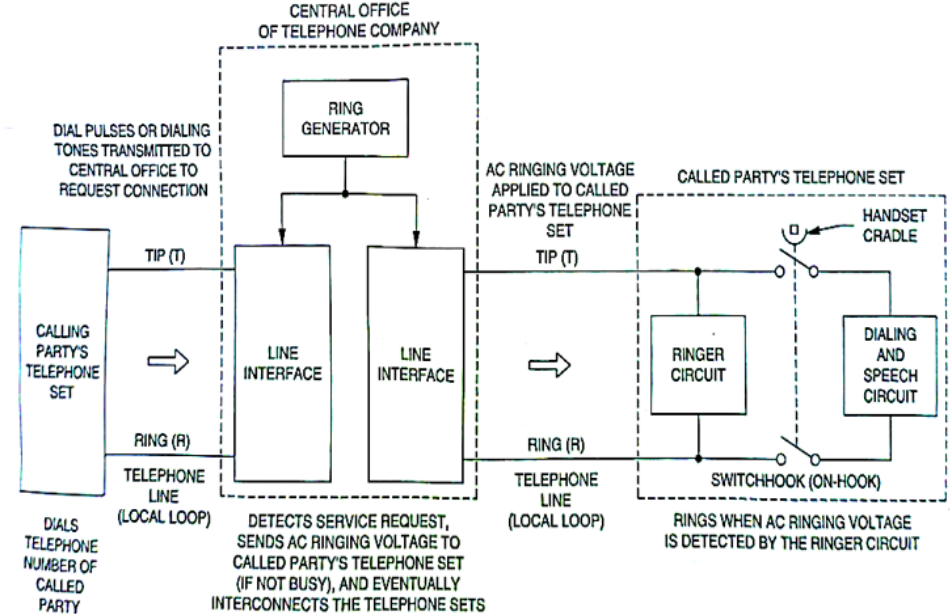
\includegraphics[width=0.68\linewidth]{Images/1}
		\caption{Making a Telephone Set Ring}
		\label{fig:ringing}
	\end{figure}
	
	Common signals in telephone networks include:
	\begin{itemize}
		\item \textbf{Dial Tone:} Continuous tone (typically 350 Hz + 440 Hz) indicating the system is ready to accept a number.
		\item \textbf{Ring Tone:} Repetitive tone (often 440 Hz + 480 Hz) heard by the caller, indicating the callee's phone is ringing.
		\item \textbf{Busy Tone:} Interrupted tone (usually 480 Hz + 620 Hz) indicating the callee's line is currently engaged.
		\item \textbf{Speech Signal:} Analog voice signal (approximately 300 Hz to 3400 Hz) transmitted and received.
	\end{itemize}
	
	Call establishment involves:
	\begin{enumerate}
		\item Lifting the handset (off-hook)
		\item Receiving the dial tone
		\item Dialing the number
		\item Enabling voice communication
	\end{enumerate}
	
	Termination occurs when the handset is placed back (on-hook), disconnecting the call.
	
	\begin{figure}[H]
		\centering
	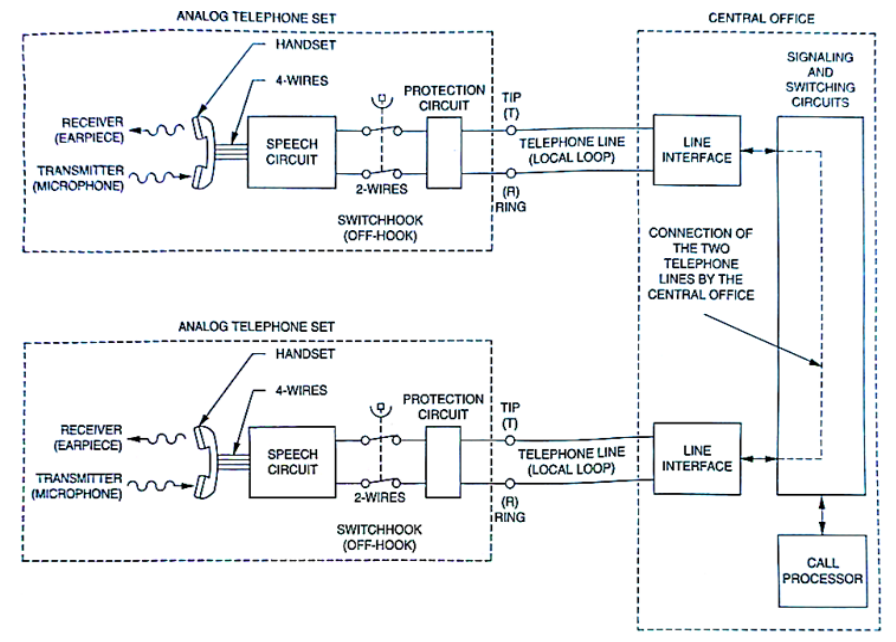
\includegraphics[width=0.71\linewidth]{Images/2}
		\caption{Two Interconnected Telephone Sets}
		\label{fig:interconnected}
	\end{figure}
	
	The speech circuit performs two-wire to four-wire (2W/4W) conversion, routing signals properly to the handset microphone and earpiece. The switchhook controls connection to the telephone line based on the handset's position.
	
	\section{Required Apparatus}
	\begin{enumerate}
		\item Telephone Set Trainer Module
		\item Two analog telephone sets
		\item Oscilloscope or signal analyzer
		\item Connecting wires
		\item Power supply unit
	\end{enumerate}
	
	\section{Experimental Setup}
	\begin{figure}[H]
		\centering
	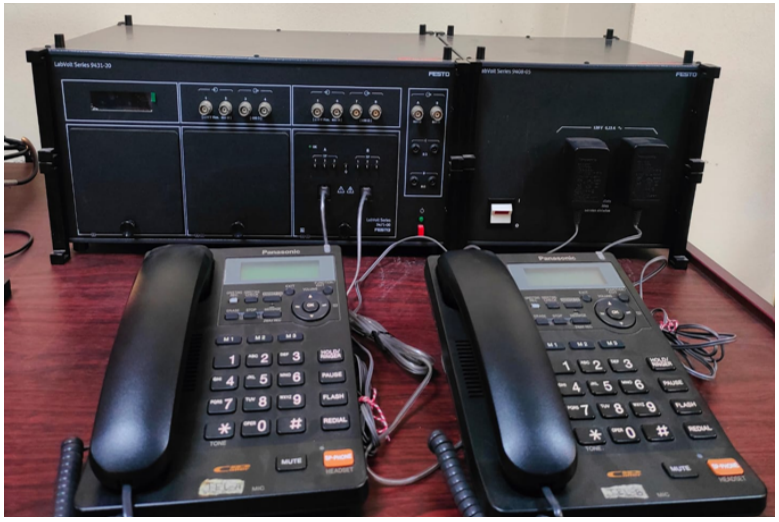
\includegraphics[width=0.68\linewidth]{Images/3}
		\caption{Experimental Setup Diagram}
		\label{fig:setup}
	\end{figure}
	
	\section{Observations}
	During the experiment, the following signals were observed and analyzed:
	
	\begin{figure}[H]
		\centering
	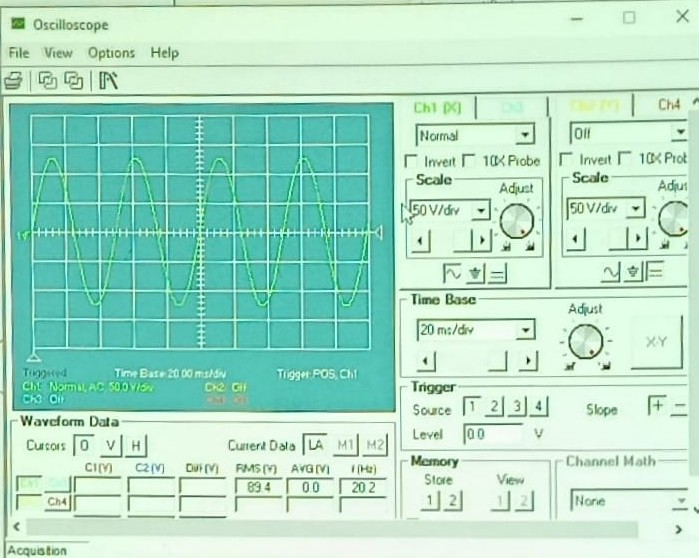
\includegraphics[width=0.68\linewidth]{Images/5}
		\caption{Signal Observation During Busy Tone}
		\label{fig:busy}
	\end{figure}
	
	\begin{figure}[H]
		\centering
	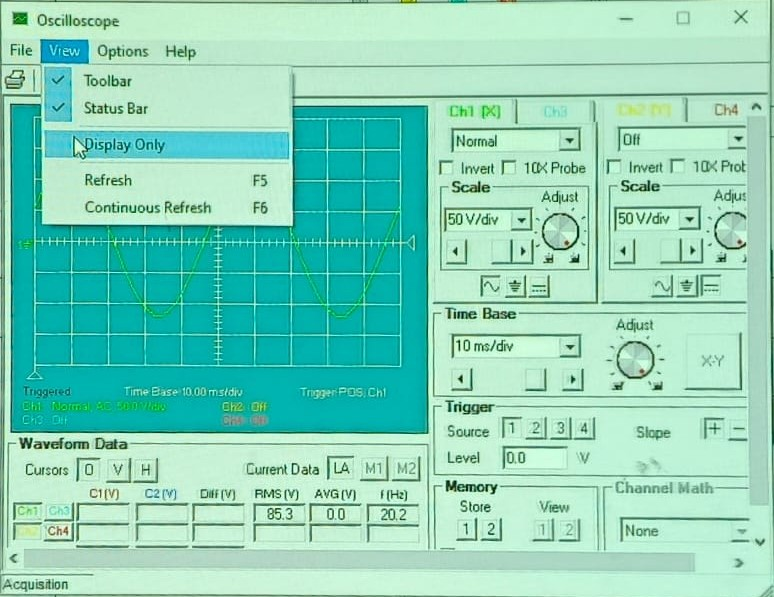
\includegraphics[width=0.68\linewidth]{Images/4}
		\caption{Signal Observation During Ringing Tone}
		\label{fig:ring}
	\end{figure}
	
	Key observations included:
	\begin{enumerate}
		\item Frequency characteristics of different tones
		\item Voltage levels of ringing signals
		\item Timing patterns of busy and ring tones
		\item Signal transformations during call establishment
	\end{enumerate}
	

	\section{Discussion}
	
	The relationship between ringing voltage and geographical standards was successfully demonstrated. In North America, the ringing signal was measured at 89.4 V (RMS) and 20 Hz, while during ring tone, 85.3 V (RMS) and 20 Hz were observed. European standards were noted to range between 16-50 Hz and 40-130 V RMS.
	
	The speech circuit's role in compensating for line attenuation was verified, and the complete call setup and termination process was successfully simulated. The Telephone Set Trainer Module was found to effectively replicate a PSTN environment, enabling clear observation of all key telephony signals.
	
	

	
\end{document}